\documentclass[tikz,border=5mm]{standalone}
\usepackage{tikz}
\usetikzlibrary{calc}

% Macro to draw perpendicular double tick marks
\newcommand{\drawticks}[4]{
    % #1 = first point, #2 = second point, #3 = tick length, #4 = spacing
    \pgfmathsetmacro{\lineangle}{atan2(#2-#1)}
    \coordinate (mid) at ($(#1)!0.5!(#2)$);
    \draw[very thick] ($(mid)+({\lineangle+90}:#3)$) -- ($(mid)+({\lineangle-90}:#3)$);
    \draw[very thick] ($(mid)+({\lineangle}:#4)+({\lineangle+90}:#3)$) -- ($(mid)+({\lineangle}:#4)+({\lineangle-90}:#3)$);
}

\begin{document}
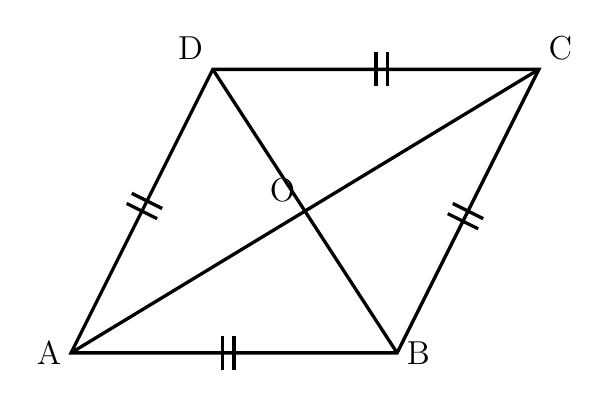
\begin{tikzpicture}[scale=1.8]

% Define vertices of rhombus
\coordinate (A) at (0,0);
\coordinate (D) at (1,2);
\coordinate (C) at (3.3,2);
\coordinate (B) at (2.3,0);

% Calculate center O
\coordinate (O) at ($(A)!0.5!(C)$);

% Draw rhombus sides
\draw[very thick] (A) -- (D) -- (C) -- (B) -- cycle;

% Draw diagonals
\draw[very thick] (A) -- (C);
\draw[very thick] (D) -- (B);

% Tick marks on AD (perpendicular)
\coordinate (midAD) at ($(A)!0.5!(D)$);
\pgfmathsetmacro{\angleAD}{atan2(2,1)}
\draw[very thick] ($(midAD)+({\angleAD+90}:0.12)$) -- ($(midAD)+({\angleAD-90}:0.12)$);
\draw[very thick] ($(midAD)+({\angleAD}:0.08)+({\angleAD+90}:0.12)$) -- ($(midAD)+({\angleAD}:0.08)+({\angleAD-90}:0.12)$);

% Tick marks on DC (perpendicular - vertical lines since DC is horizontal)
\coordinate (midDC) at ($(D)!0.5!(C)$);
\draw[very thick] ($(midDC)+(90:0.12)$) -- ($(midDC)+(-90:0.12)$);
\draw[very thick] ($(midDC)+(0:0.08)+(90:0.12)$) -- ($(midDC)+(0:0.08)+(-90:0.12)$);

% Tick marks on CB (perpendicular)
\coordinate (midCB) at ($(C)!0.5!(B)$);
\pgfmathsetmacro{\angleCB}{atan2(-2,-1)}
\draw[very thick] ($(midCB)+({\angleCB+90}:0.12)$) -- ($(midCB)+({\angleCB-90}:0.12)$);
\draw[very thick] ($(midCB)+({\angleCB}:0.08)+({\angleCB+90}:0.12)$) -- ($(midCB)+({\angleCB}:0.08)+({\angleCB-90}:0.12)$);

% Tick marks on BA (perpendicular - vertical lines since BA is horizontal)
\coordinate (midBA) at ($(B)!0.5!(A)$);
\draw[very thick] ($(midBA)+(90:0.12)$) -- ($(midBA)+(-90:0.12)$);
\draw[very thick] ($(midBA)+(180:0.08)+(90:0.12)$) -- ($(midBA)+(180:0.08)+(-90:0.12)$);

% Vertex labels
\node[left] at (A) {\large A};
\node[above left] at (D) {\large D};
\node[above right] at (C) {\large C};
\node[right] at (B) {\large B};
\node[above left] at (O) {\large O};

\end{tikzpicture}
\end{document}